\documentclass[aspectratio=169]{beamer}
\usepackage[utf8]{inputenc}
\usepackage{hyperref}
\usepackage{amsmath,amsfonts,amsthm,bm}
\usepackage{color}
\usepackage{minted}
\usepackage{graphicx} % Allows including images
\usepackage{booktabs} % Allows the use of \toprule, \midrule and \bottomrule in tables
\usepackage{tikz}
\usepackage[version=3]{mhchem}
\usepackage{pgfplots}
\pgfplotsset{compat=1.16}
\setminted{fontsize=\scriptsize}


\hypersetup{
    colorlinks=true,
    linkcolor=red,
    filecolor=magenta,
    urlcolor=red,
}

\DeclareMathOperator*{\argmax}{argmax}
\DeclareMathOperator*{\argmin}{argmin}
\let \vec \mathbf

\newcommand{\classname}{NANOx81R}
\usetheme{metropolis}

\setbeamerfont{frametitle}{size=\Large,series=\bfseries}
\metroset{block=fill}


\title[Introduction to Data Science in Materials Science]{Introduction to Data Science in Materials Science}

\author{Shyue Ping Ong}
\institute[UCSD]{Aiiso Yufeng Li Family Department of Chemical and Nano Engineering\\
University of California, San Diego\\\url{http://materialsvirtuallab.org}}
\date{}

\begin{document}


    \begin{frame}
        \titlepage % Print the title page as the first slide
    \end{frame}


    \begin{frame}{What is Data Science?}
        \Large{Data science is a multi-disciplinary field that uses scientific methods, processes, algorithms and systems to \textcolor{red}{extract knowledge and insights from structured and unstructured data}.}
    \end{frame}


    \begin{frame}{What is Data Science?}
        \begin{figure}
            \centering
            \includegraphics[width=0.5\textwidth]{figures/datascience.png}
        \end{figure}
    \end{frame}

    \begin{frame}{The Data Age}
        \begin{figure}
            \centering
            \includegraphics[width=0.6\textwidth]{figures/worldwidedatacreation.png}
        \end{figure}
    \end{frame}

    \begin{frame}{Growth in Materials Data (as of Jan 1 2020)}

        \begin{columns}
            \column{0.5\textwidth}
            \begin{figure}
                \centering
                \includegraphics[width=0.45\textwidth]{figures/icsd.png}
                \caption{ICSD: $\sim$200,000 crystals
                }
            \end{figure}
            \begin{figure}
                \centering
                \includegraphics[width=0.45\textwidth]{figures/cod.png}
                \caption{COD: $\sim$400,000 crystals
                }
            \end{figure}

            \column{0.5\textwidth}
            \begin{figure}
                \centering
                \includegraphics[width=0.45\textwidth]{figures/pdb.png}
                \caption{Protein data bank}
            \end{figure}
            \begin{figure}
                \centering
                \includegraphics[width=0.45\textwidth]{figures/csd.png}
                \caption{Cambridge structural database (small-molecule organic crystal structures)}
            \end{figure}
        \end{columns}
    \end{frame}


    \begin{frame}{But Quantity and Quality Lags Many Other Fields}

        \begin{columns}
            \column{0.5\textwidth}
            \begin{figure}
                \centering
                \includegraphics[width=0.45\textwidth]{figures/handbook_of_condensed_matter.jpg}
                \caption{One of the most comprehensive handbooks on materials data: Density, thermal and electrical conductivity, melting and boiling points, etc., but O(100) binaries and limited ternaries...
                }
            \end{figure}
            \column{0.5\textwidth}
            \begin{figure}
                \centering
                \includegraphics[width=0.9\textwidth]{figures/supercon.png}
                \caption{$\sim$1000+ superconductors (many minor composition modifications). Ref: \url{ https://supercon.nims.go.jp/}
                }
            \end{figure}
        \end{columns}
    \end{frame}

    \begin{frame}{First Principles Materials Computations}
        \begin{figure}
            \centering
            \includegraphics[width=0.7\textwidth]{figures/computational_materials_science.png}
        \end{figure}
    \end{frame}

    \begin{frame}{Electronic structure calculations are today \textit{reliable} and \textit{reasonably accurate}...}

        \begin{columns}
            \column{0.2\textwidth}
            \begin{figure}
                \centering
                \includegraphics[width=\textwidth]{figures/reliability_of_dft.png}
            \end{figure}
            \column{0.5\textwidth}
            \begin{figure}
                \centering
                \includegraphics[width=0.45\textwidth]{figures/icsd_e_hull.png}
                \includegraphics[width=0.45\textwidth]{figures/formation_energies.png}\\
                \includegraphics[width=0.45\textwidth]{figures/surface_energies.png}
                \includegraphics[width=0.45\textwidth]{figures/elastic_constants.png}
            \end{figure}
            \column{0.2\textwidth}
            \begin{itemize}
                \tiny
                \item (left) Modern electronic structure codes give relatively consistent equations of state.
                \item (right, clockwise from top left) Good predictions can be obtained for phase stability,\cite{sunThermodynamicScaleInorganic2016} formation energies, surface energies,\cite{tranSurfaceEnergiesElemental2016} and elastic constants\cite{dejongChartingCompleteElastic2015}.
            \end{itemize}
        \end{columns}
    \end{frame}

    \begin{frame}{Software frameworks for high-throughput computational materials science}
        \begin{itemize}
            \item Materials Project (\url{https://materialsproject.org})\cite{jainCommentaryMaterialsProject2013}
            \begin{itemize}
                \item Python Materials Genomics or pymatgen (\url{https://pymatgen.org})\cite{ongPythonMaterialsGenomics2013}
                \item Custodian (\url{https://materialsproject.github.io/custodian/})
                \item FireWorks \cite{jainFireWorksDynamicWorkflow2015}
            \end{itemize}
            \item Atomic Simulation Environment (\url{https://wiki.fysik.dtu.dk/ase})
            \item AFLOW (\url{http://aflowlib.org})\cite{curtaroloAFLOWLIBORGDistributed2012}
            \item AiiDa (\url{http://www.aiida.net})
        \end{itemize}
    \end{frame}


    \begin{frame}{Computation + Automation $\rightarrow$ Large databases}
        \begin{figure}
            \centering
            \includegraphics[width=0.7\textwidth]{figures/materials_databases.png}
        \end{figure}
    \end{frame}


    \begin{frame}{Google for Materials}
        \begin{figure}
            \centering
            \includegraphics[width=0.45\textwidth]{figures/mgi.png}
            \includegraphics[width=0.25\textwidth]{figures/doe_mp.png}
        \end{figure}
        \includegraphics[width=0.1\textwidth]{figures/mp_logo.png}
        The Materials Project is an open science project to make the computed properties of all known inorganic materials publicly available to all researchers to accelerate materials innovation.
    \end{frame}


    \begin{frame}{Google for Materials}
        \begin{figure}
            \centering
            \includegraphics[width=0.40\textwidth]{figures/mp_image1.png}
            \includegraphics[width=0.20\textwidth]{figures/mp_image2.png}
        \end{figure}
    \end{frame}


    \begin{frame}{Materials Application Programming Interface (API)\cite{ongMaterialsApplicationProgramming2015}}
        \begin{itemize}
            \item An open platform for accessing Materials Project data based on REpresentational State Transfer (REST) principles.
            \item \textit{Flexible and scalable} to cater to large number of users, with different access privileges.
            \item Simple to use and code agnostic.
            \item Requires an API key, available at: \url{https://www.materialsproject.org/dashboard}
            \item Documentation: \url{https://api.materialsproject.org/docs}
        \end{itemize}
    \end{frame}


    \begin{frame}{RESTful API}
        A REST API maps a URL to a resource.
        \begin{exampleblock}{Example}
            GET https://api.dropbox.com/1/account/info
        \end{exampleblock}
        Returns information about a user’s account.

        Methods: GET, POST, PUT, DELETE, etc.

        Response: Usually JSON or XML or both
    \end{frame}


    \begin{frame}{Materials API Example}
        \begin{exampleblock}{URL}
            \footnotesize
            \textcolor{red}{https://api.materialsproject.org}/\textcolor{blue}{summary}/?\textcolor{green}{formula=Fe2O3}\&\_fields=formation\_energy\_per\_atom\\
        \end{exampleblock}
        \begin{columns}
            \column{0.4\textwidth}
            Example response:
            \inputminted{json}{mapi_response.txt}
            \column{0.45\textwidth}
            \begin{itemize}
                \item[]
                \item[]
                \item[]
                \item Intuitive response format.
                \item Machine-readable (JSON parsers available for most programming languages).
                \item Metadata provides provenance for tracking.
            \end{itemize}
        \end{columns}
    \end{frame}


    \begin{frame}[t]{Types of Materials Data}
        \begin{columns}[t]
            \column{0.33\textwidth}
            \begin{exampleblock}{Qualitative data}
                \begin{itemize}
                    \item Nominal measurement.
                    \item E.g., Metal/Insulator, Stable/Unstable.
                    \item No rank or order.
                \end{itemize}
            \end{exampleblock}
            \column{0.33\textwidth}
            \begin{exampleblock}{Ranked data}
                \begin{itemize}
                    \item Ordinal measurement (ordered).
                    \item E.g., Insulator/ semiconductor/ conductor.
                    \item Does not indicate distance between ranks.
                \end{itemize}
            \end{exampleblock}
            \column{0.33\textwidth}
            \begin{exampleblock}{Quantitative Data
            }
                \begin{itemize}
                    \item Interval/ratio measurement (equal intervals and true 0).
                    \item E.g., melting point, elastic constant, electrical/ionic conductivity.
                    \item Considerable information and permits meaningful arithmetic operations.
                \end{itemize}
            \end{exampleblock}
        \end{columns}
    \end{frame}

    \begin{frame}{What is Machine Learning?}
        \begin{columns}
            \column{0.5\textwidth}
            \begin{figure}
                \centering
                \includegraphics[width=\textwidth]{figures/ml.png}
            \end{figure}
            \column{0.5\textwidth}
            \begin{figure}
                \centering
                \includegraphics[width=0.49\textwidth]{figures/waymo.png}
                \includegraphics[width=0.49\textwidth]{figures/alphago.jpeg}
                \includegraphics[width=0.49\textwidth]{figures/netflixrec.png}
            \end{figure}
        \end{columns}


    \end{frame}

    \begin{frame}{Nobel Prizes in Chemistry and Physics 2024}
        \begin{figure}
            \centering
            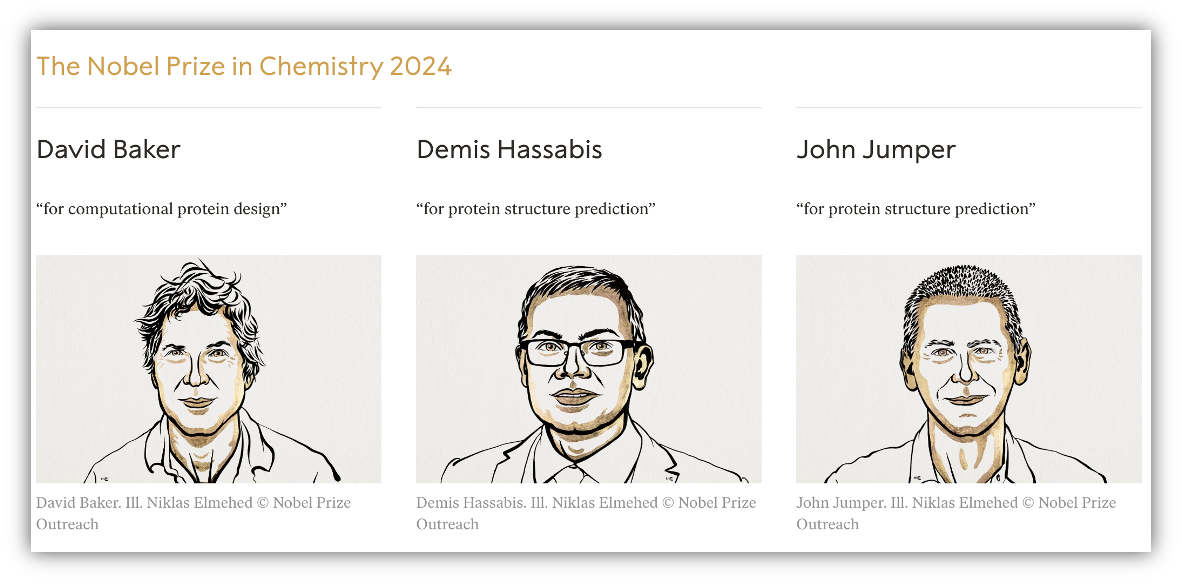
\includegraphics[width=0.6\textwidth]{lectures/slides_tex/figures/nobel-chem-2024.png}
            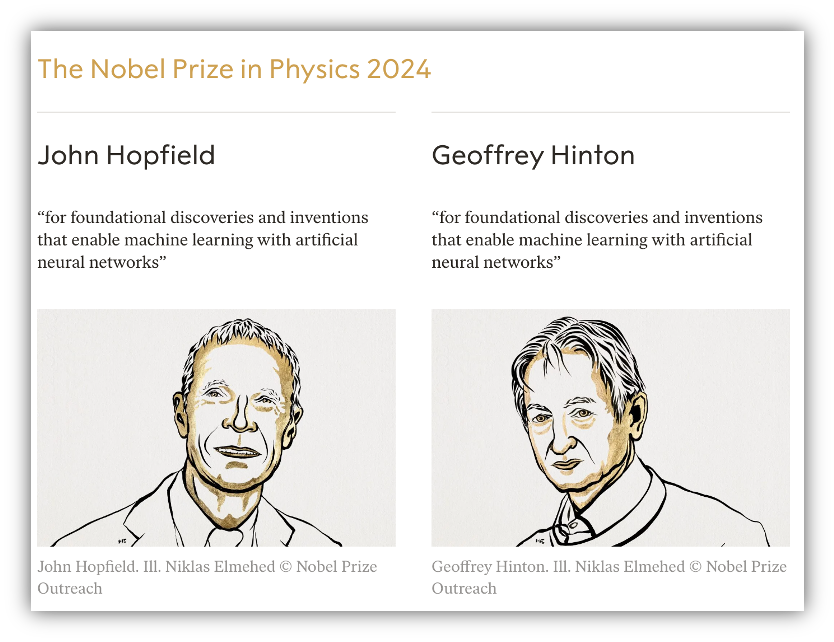
\includegraphics[width=0.38\textwidth]{lectures/slides_tex/figures/nobel-physics-2024.png}
        \end{figure}
    \end{frame}


    \begin{frame}[t]{Materials ML Workflow}
        \begin{figure}
            \centering
            \includegraphics[width=0.7\textwidth]{figures/materials_ml_workflow.pdf}
        \end{figure}
    \end{frame}


    \begin{frame}[t]{Where is ML valuable in Materials Science?}
        \begin{columns}[t]
            \column{0.33\textwidth}
            Too many to compute
            \begin{figure}
                \centering
                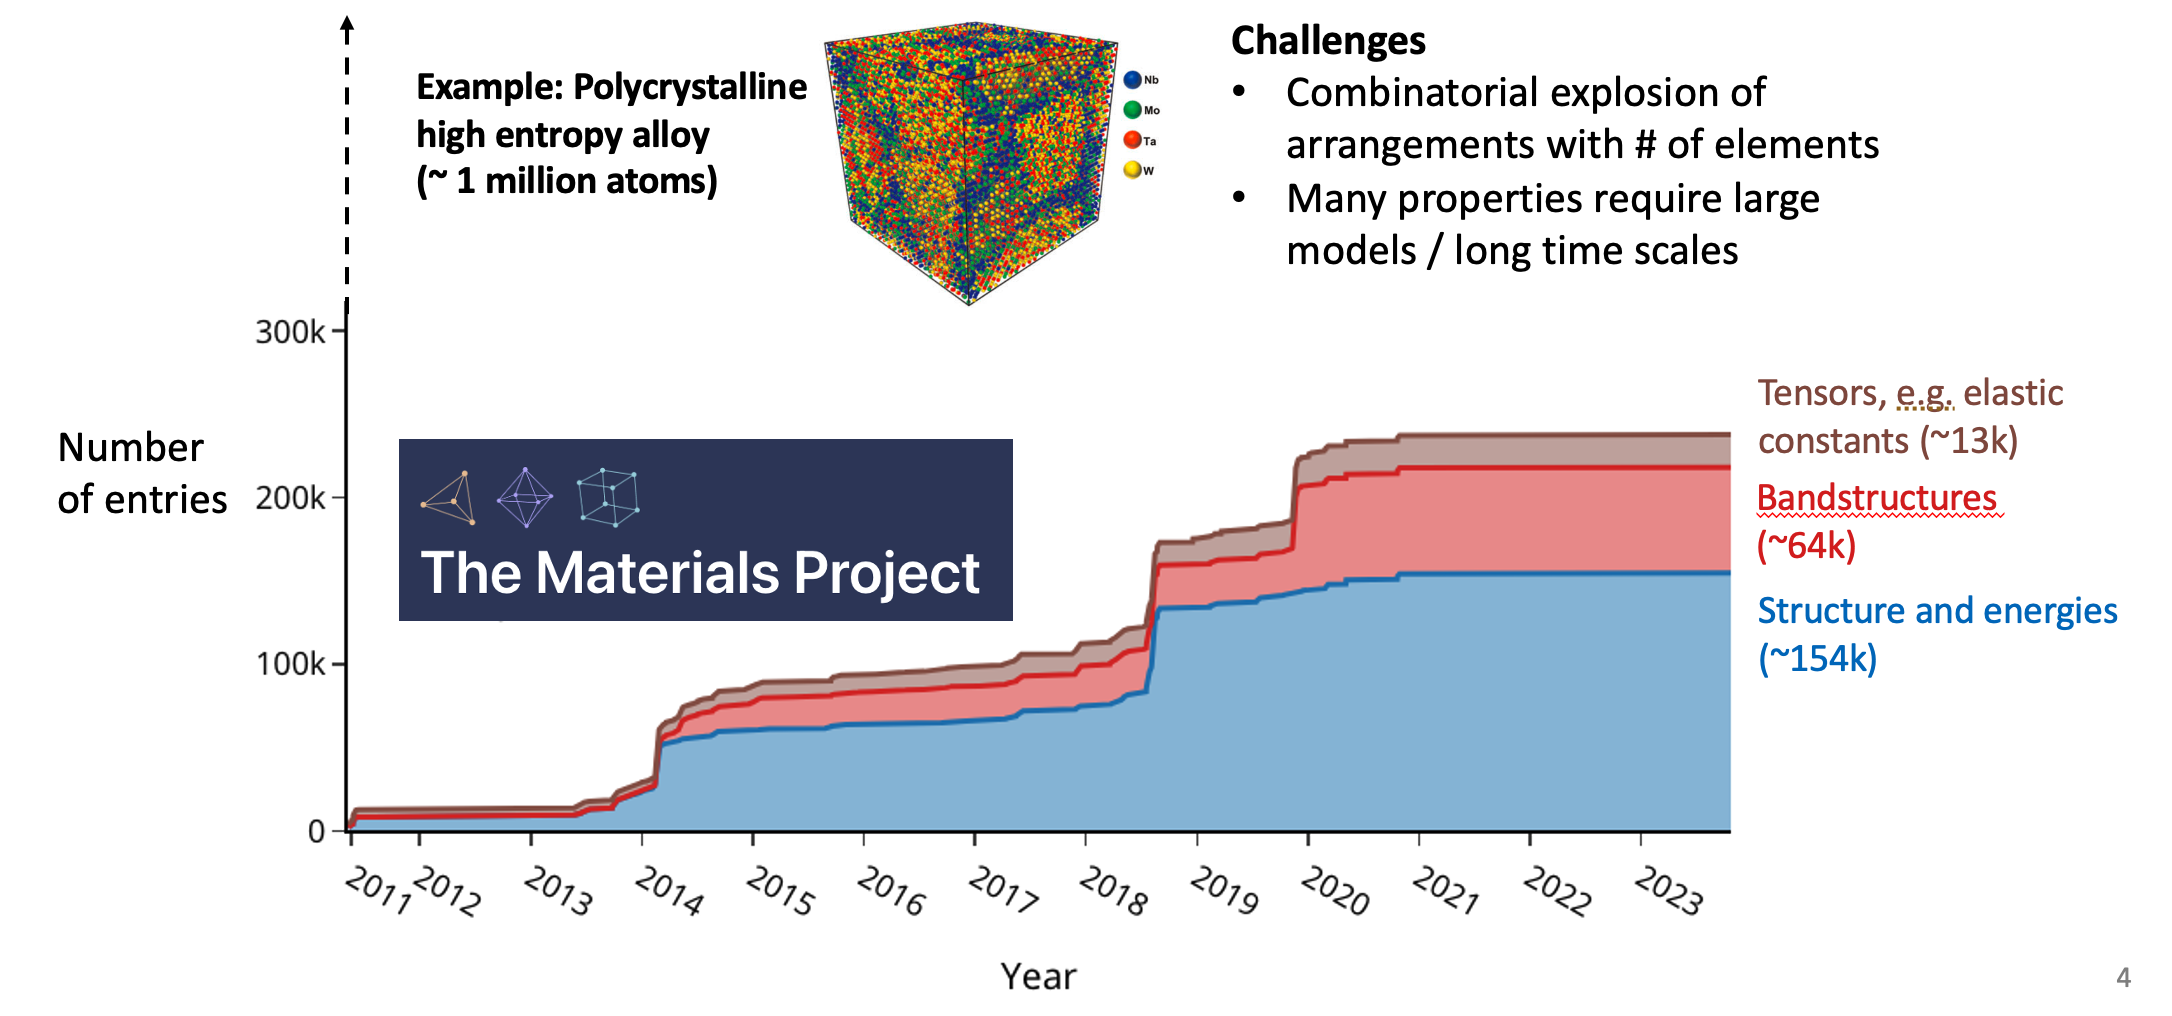
\includegraphics[width=\textwidth]{figures/mp_data_hist.png}
            \end{figure}
            \column{0.33\textwidth}
            Too big to compute
            \begin{figure}
                \centering
                \includegraphics[width=\textwidth]{figures/mpea_poly.png}
            \end{figure}
            \column{0.33\textwidth}
            Too complex to understand.
            \begin{figure}
                \centering
                \includegraphics[width=0.7\textwidth]{figures/xas_interpretation.png}
            \end{figure}
        \end{columns}
    \end{frame}


    \begin{frame}{Data History of the Materials Project}
        \begin{figure}
            \centering
            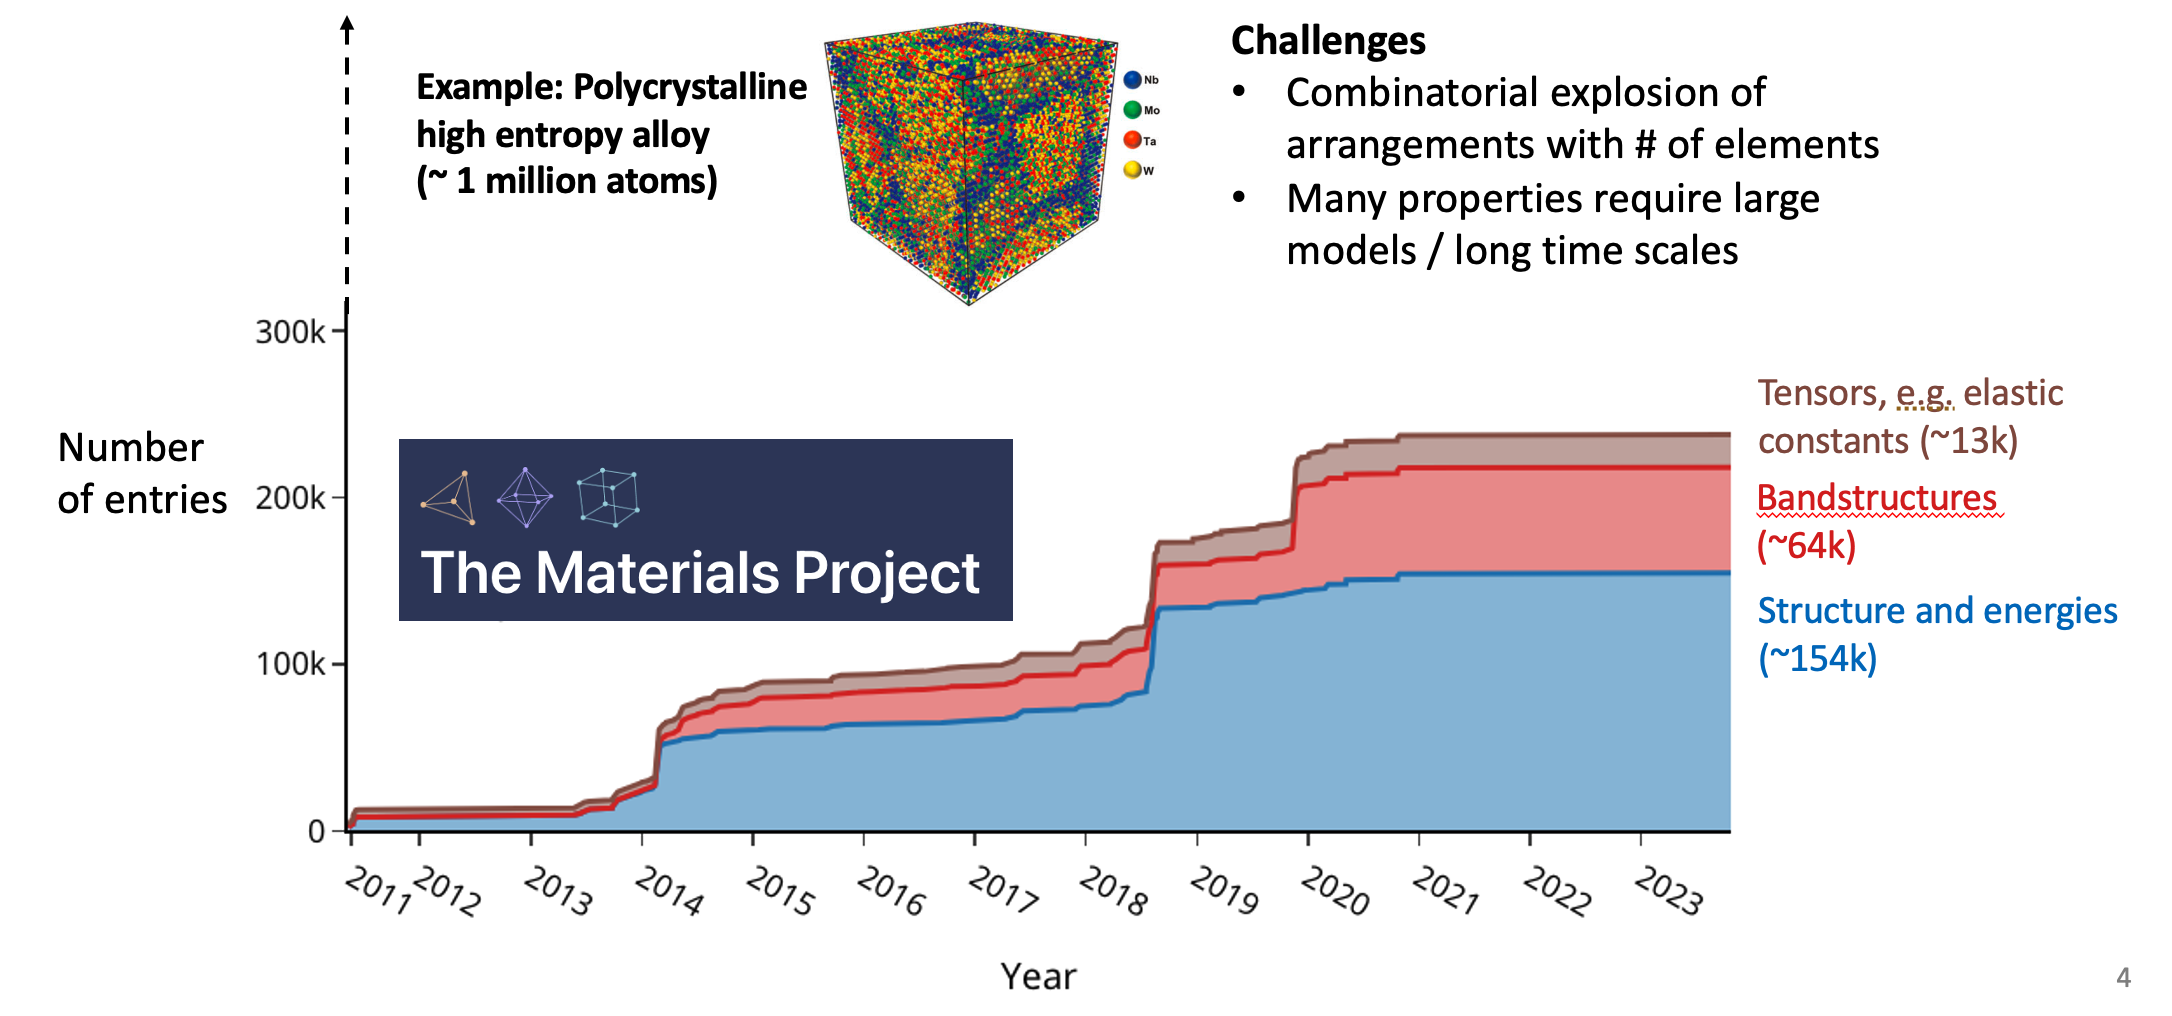
\includegraphics[width=0.8\textwidth]{figures/mp_data_hist.png}
        \end{figure}
    \end{frame}


    \begin{frame}{Surrogate models for “instant” property predictions}
        \begin{equation*}
            \mathrm{Property} = f(\mathrm{Composition}, \mathrm{Structure})
        \end{equation*}
        \begin{itemize}
            \item The material property, e.g., energetic (formation, energy above hull, reaction, etc.), electronic (band gaps, DOS), mechanical, functional (e.g., ionic conductivity) is called the \textbf{``target''}.
            \item Composition and Structure are called the \textbf{``descriptors''} or \textbf{``features''}.
            \item Examples of compositonal features: stoichiometric attributes, e.g., \# and ratio of elements; elemental properties, e.g., mean, range, min, max of atomic number, electronegativity, row, group, radii, \# of valence electrons, etc.
            \item Examples of structural features: crystal/molecular symmetry, lattice parameters, atomic coordinates, connectivity / bonding between atoms.
        \end{itemize}
    \end{frame}


    \begin{frame}{Compositional features}

        \begin{columns}
            \column{0.25\textwidth}
            \begin{figure}
                \centering
                \includegraphics[width=\textwidth]{figures/compositional_features.png}
                \caption{Meredig et al. (2014) Phys. Rev. B89, 094104}
            \end{figure}
            \column{0.75\textwidth}
            \begin{figure}
                \centering
                \includegraphics[width=0.49\textwidth]{figures/elemnet.png}
                \includegraphics[width=0.49\textwidth]{figures/compositional_cnn.png}
                \caption{Jha et al. (2018) Sci. Rep., 8(1), 17593., Zheng, X., et al (2018). Chem. Sci., 9(44), 8426-8432.}
            \end{figure}
        \end{columns}
    \end{frame}


    \begin{frame}{Structural features}
        \begin{columns}
            \column{0.33\textwidth}
            \begin{figure}
                \centering
                \includegraphics[width=\textwidth]{figures/fragments_gb.png}
                \caption{Property-labelled materials fragments + gradient boosting decision tree.\cite{isayevUniversalFragmentDescriptors2016}}
            \end{figure}
            \column{0.33\textwidth}
            \begin{figure}
                \centering
                \includegraphics[width=\textwidth]{figures/cgcnn.png}
                \caption{Crystal graph + graph convolutional neural networks}
            \end{figure}
            \column{0.33\textwidth}
            \begin{figure}
                \centering
                \includegraphics[width=\textwidth]{figures/soap.png}
                \caption{Smooth overlap of atom positions (SOAP).\cite{rosenbrockDiscoveringBuildingBlocks2017}}
            \end{figure}
        \end{columns}
    \end{frame}


    \begin{frame}{Example: Graph-based representations}
        \begin{figure}
            \centering
            \includegraphics[width=0.45\textwidth]{figures/model_diagram.png}
            \includegraphics[width=0.45\textwidth]{figures/model_arch.jpg}
            \caption{MatErials Graph Networks (MEGNet).\cite{chenGraphNetworksUniversal2019}}
        \end{figure}
    \end{frame}


    \begin{frame}{MEGNet Performance Benchmarks}
        \footnotesize
        \begin{table}[]
            \centering
            \begin{tabular}{l|c|c|c}
                Property                          & MEGNet          & SchNet & CGCNN          \\
                \hline
                Formation energy $E_f$ (meV/atom) & 28 (60,000)     & 35     & 39 (28,046)    \\
                Band gap $E_g$ (eV)               & 0.330 (36,720)  & -      & 0.388 (16,485) \\
                $\log_{10} K_{VRH}$ (GPa)         & 0.050 (4,664)   & -      & 0.054 (2,041)  \\
                $\log_{10} G_{VRH}$ (GPa)         & 0.079 (4,664)   & -      & 0.087 (2,041)  \\
                Metal classifier                  & 78.9\% (55,391) & -      & 80\% (28,046)  \\
                Non-metal classifier              & 90.6\% (55,391) & -      & 95\% (28,046)
            \end{tabular}
            \caption{Materials Project Crystals. Brackets indicate number of data points.}
        \end{table}
    \end{frame}


    \begin{frame}{Scale Challenge in Materials Science}
        \begin{figure}
            \centering
            \includegraphics[width=0.7\textwidth]{figures/scale_challenge.png}
        \end{figure}
    \end{frame}


    \begin{frame}{ML Interatomic Potentials as a solution to the scale challenge}
        \begin{columns}
            \column{0.3\textwidth}
            \begin{figure}
                \centering
                \includegraphics[width=\textwidth]{figures/ML-IAP.jpg}
            \end{figure}
            \column{0.7\textwidth}
            \begin{itemize}
                \small
                \item Examples: Neural Network Potential (NNP)\cite{behlerHighDimensionalNeuralNetwork}, Gaussian Approximation Potential (GAP)\cite{bartokGaussianApproximationPotentials2010}, moment tensor potential (MTP)\cite{novikovMLIPPackageMoment2021}, spectral neighbor analysis potential,\cite{thompsonSpectralNeighborAnalysis2015}, atomic cluster expansion\cite{drautzAtomicClusterExpansion2020}, etc.
                \item ML models: Linear regression, Gaussian kernels, neural networks, etc.
                \item Local environment descriptors:
                \tiny{
                    \begin{equation*}
                        G_{i}^{\rm atom, \rm rad} = \sum_{j\neq i}^{N_{\rm atom}} e^{-\eta(R_{ij}-R_{s})^{2}} \cdot f_{c}(R_{ij}),
                    \end{equation*}
                    \begin{equation*}
                        \begin{split}
                            G_{i}^{\rm atom, \rm ang}&=2^{1-\zeta}\sum_{j,k \neq i}^{N_{\rm atom}} (1 + \lambda \cos \theta_{ijk})^{\zeta} \cdot e^{-\eta^{\prime}(R_{ij}^{2}+R_{ik}^{2}+R_{jk}^{2})}
                            \cdot f_{c}(R_{ij}) \cdot f_{c}(R_{ik}) \cdot f_{c}(R_{jk}),
                        \end{split}
                    \end{equation*}}
                \begin{equation*}
                    \rho_{i}(\boldsymbol{R}) = \sum_{j} f_{c}(R_{ij}) \cdot \exp(-\frac{|\boldsymbol{R} - \boldsymbol{R}_{ij}|^{2}}{2\sigma_{\rm atom}^{2}}),
                \end{equation*}

            \end{itemize}
        \end{columns}

    \end{frame}


    \begin{frame}{Automatable workflows for MLIP Construction}
        \begin{figure}
            \centering
            \includegraphics[width=0.45\textwidth]{figures/mliapworkflow.pdf}
            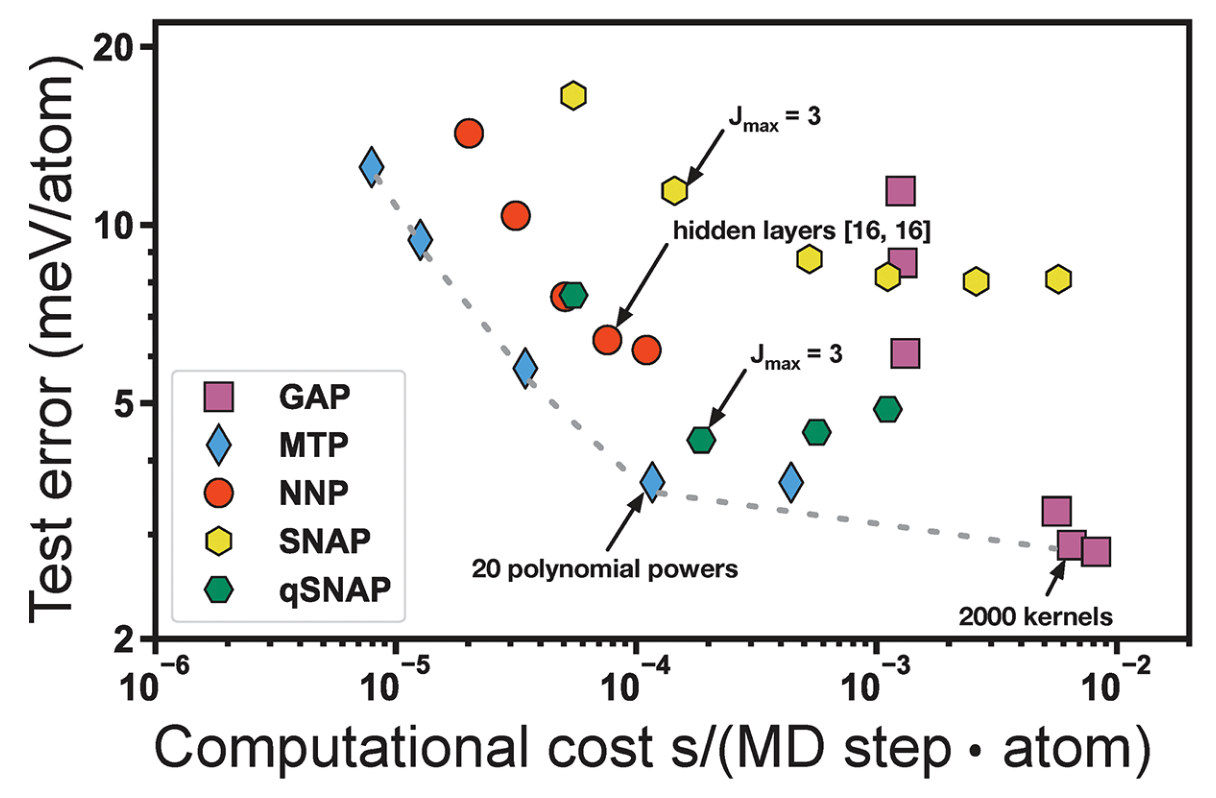
\includegraphics[width=0.45\textwidth]{figures/mliapcostvsperformance.png}
            \caption{Automatic workflow for ML-IAP construction and performance benchmarks.\cite{zuoPerformanceCostAssessment2020}}
        \end{figure}
    \end{frame}


    \begin{frame}{Example: Ni-Mo}
        \begin{figure}
            \centering
            \includegraphics[width=0.3\textwidth]{figures/ni-mo_pd.png}
            \includegraphics[width=0.35\textwidth]{figures/ni-mo-stress-strain.png}
            \caption{MLIP results on Ni-Mo. (left) Ni-Mo phase diagram. (right) Stress-strain curves as a function of grain size\cite{zuoPerformanceCostAssessment2020}}
        \end{figure}
    \end{frame}

    \begin{frame}{Universal MLIPs}
        \begin{figure}
            \centering
            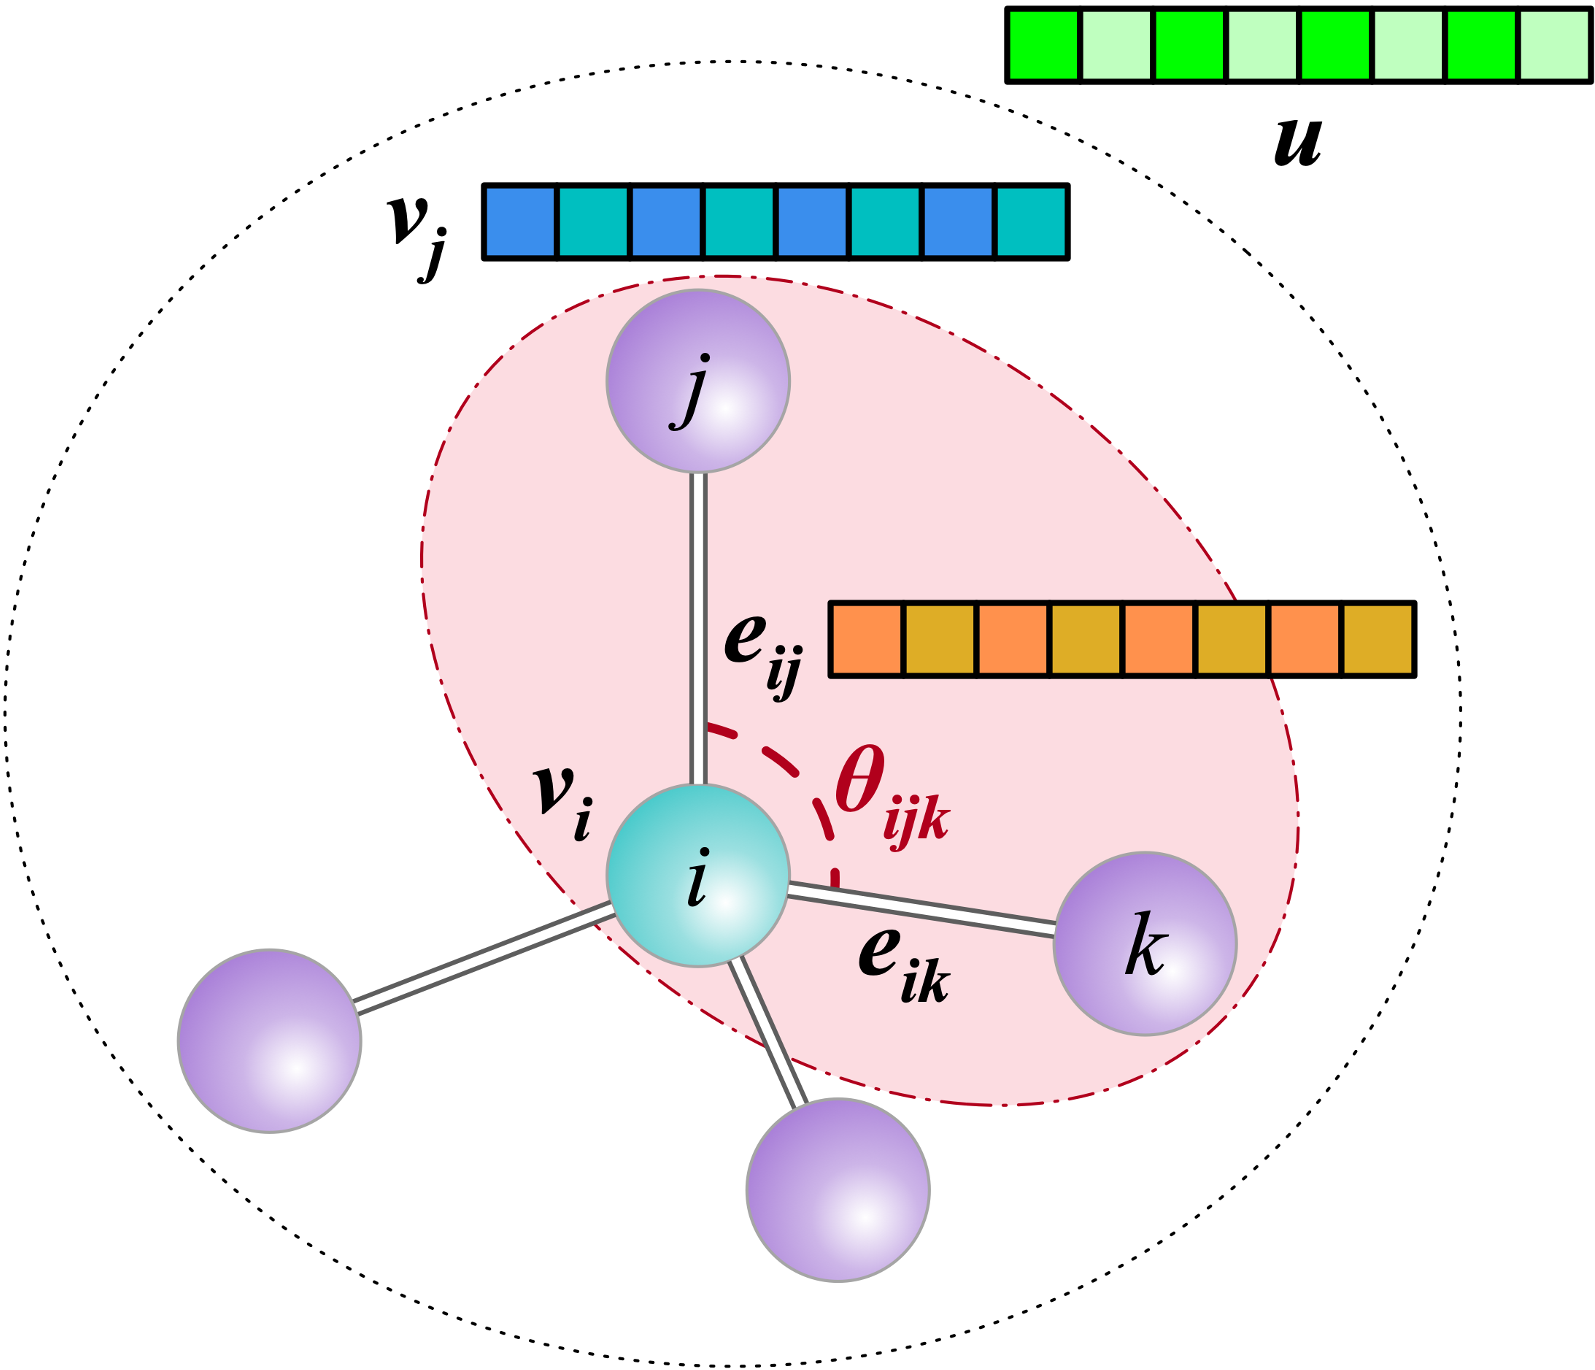
\includegraphics[width=0.4\textwidth]{figures/m3gnet.png}
            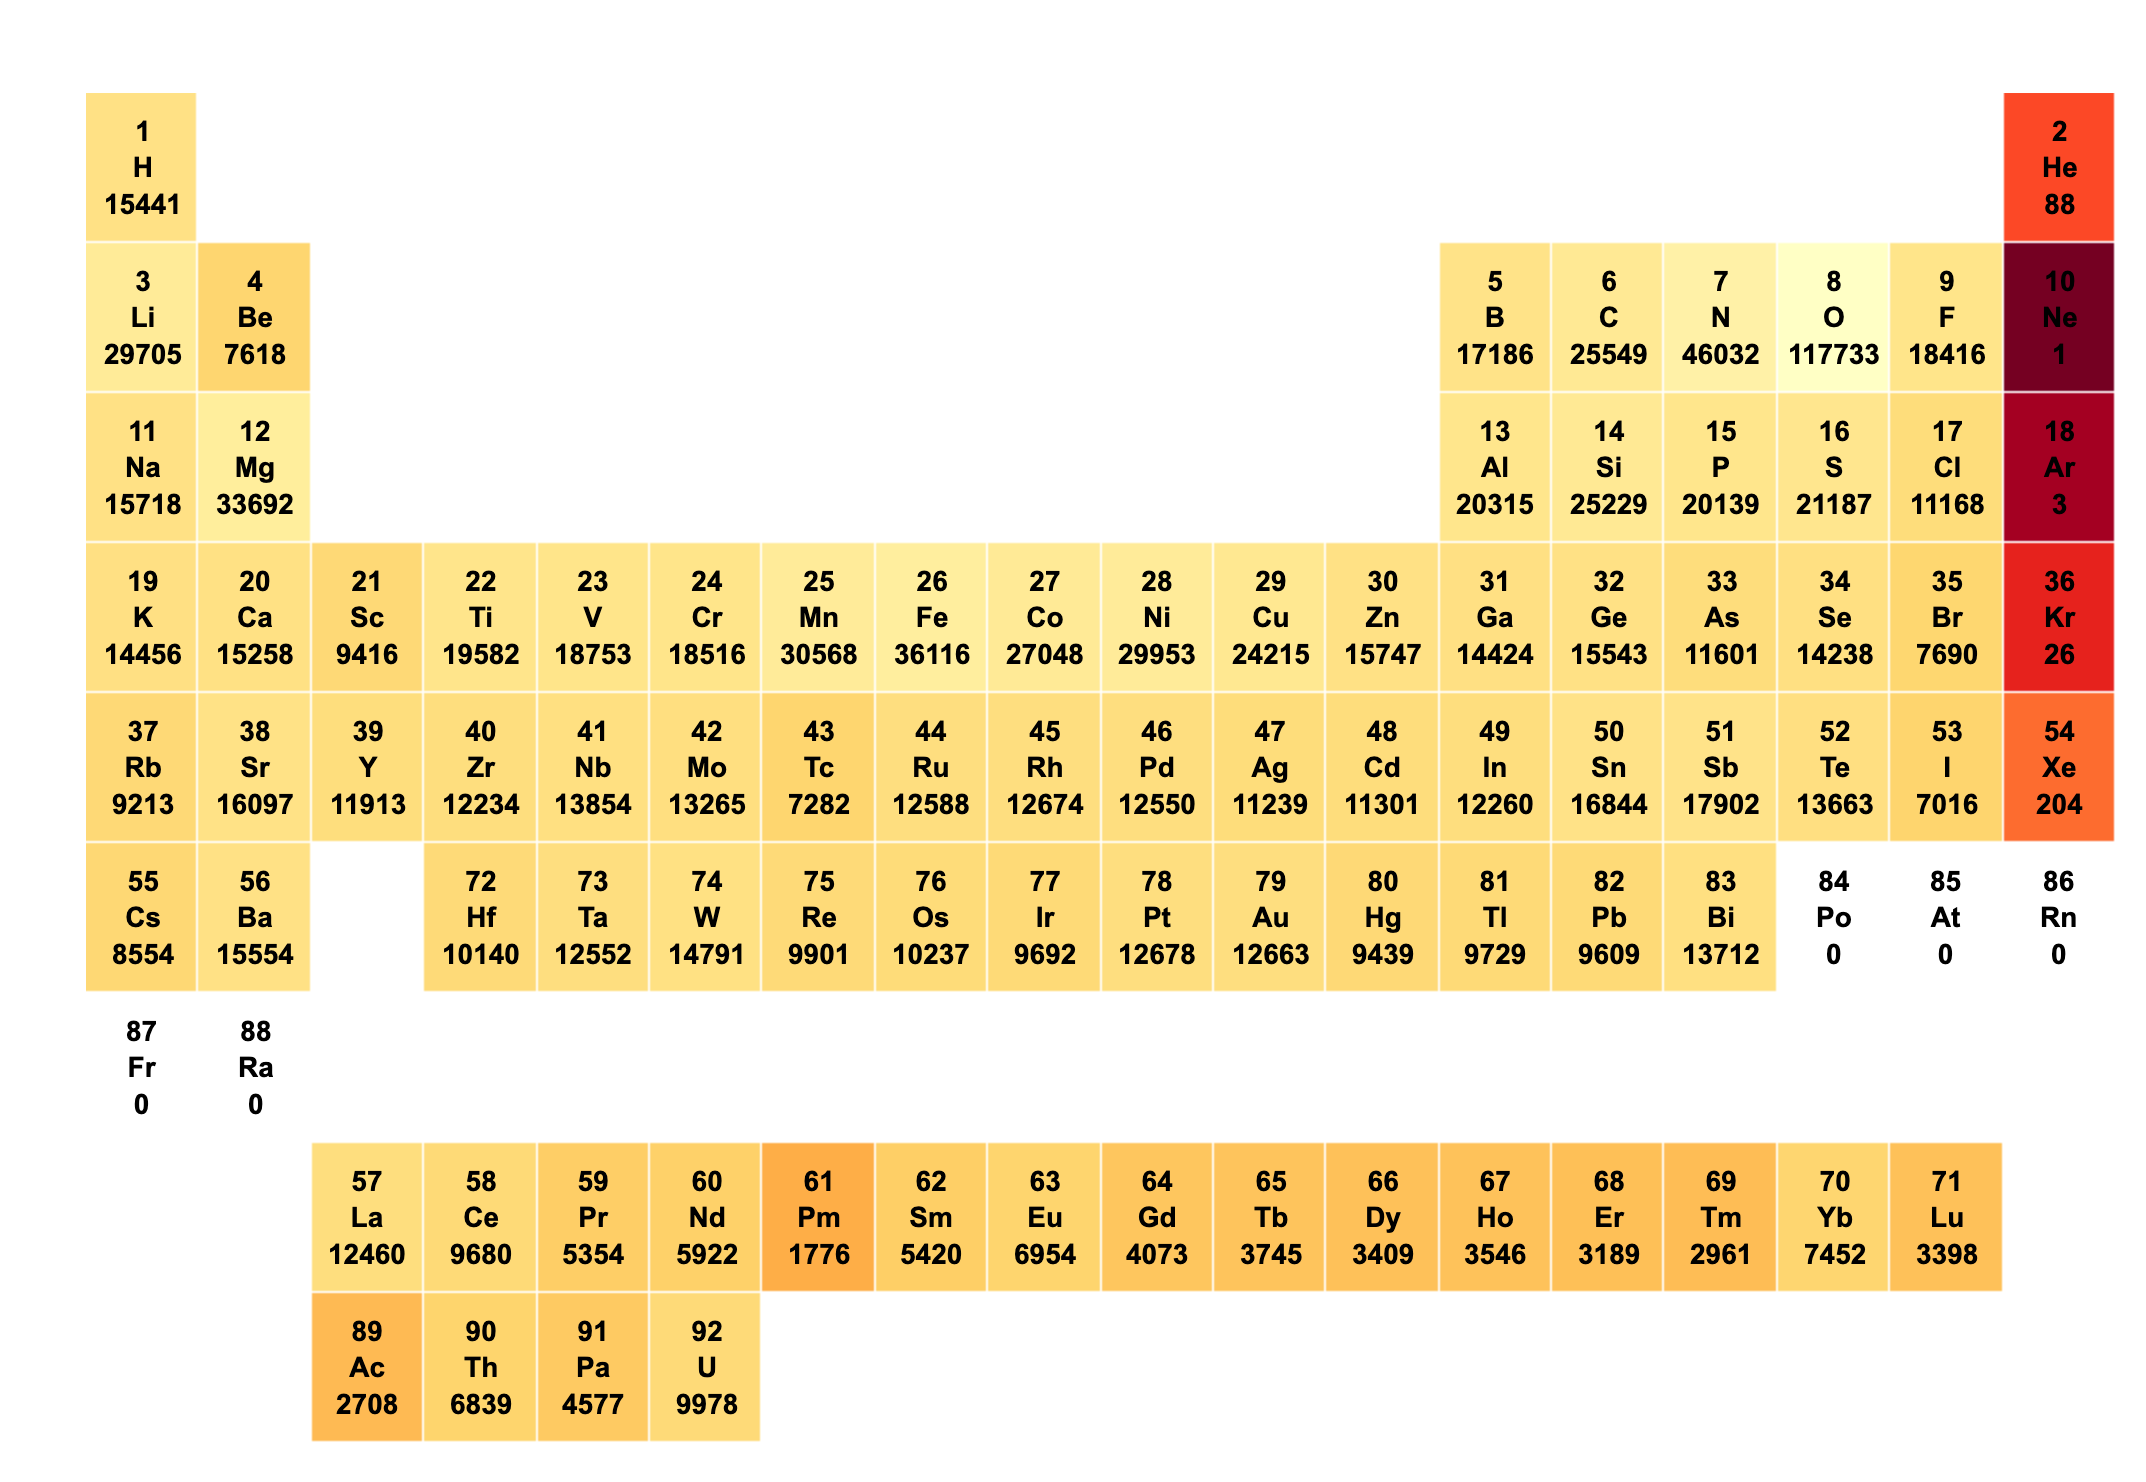
\includegraphics[width=0.5\textwidth]{lectures/slides_tex/figures/matpes-pbe-pt.png}
            \caption{Materials 3-body Graph Network (M3GNet), the first whole periodic table MLIP.\cite{chenUniversalGraphDeep2022}}
        \end{figure}
    \end{frame}


    \begin{frame}{Modeling complex relationships}
        \begin{figure}
            \centering
            \includegraphics[width=0.4\textwidth]{figures/imagenet.png}
            \includegraphics[width=0.55\textwidth]{figures/imagenetperf.png}
            \caption{ImageNet (\url{https://www.image-net.org/})}
        \end{figure}
    \end{frame}


    \begin{frame}{Example: Coordination environment from X-ray Absorption Spectra}
        \begin{figure}
            \centering
            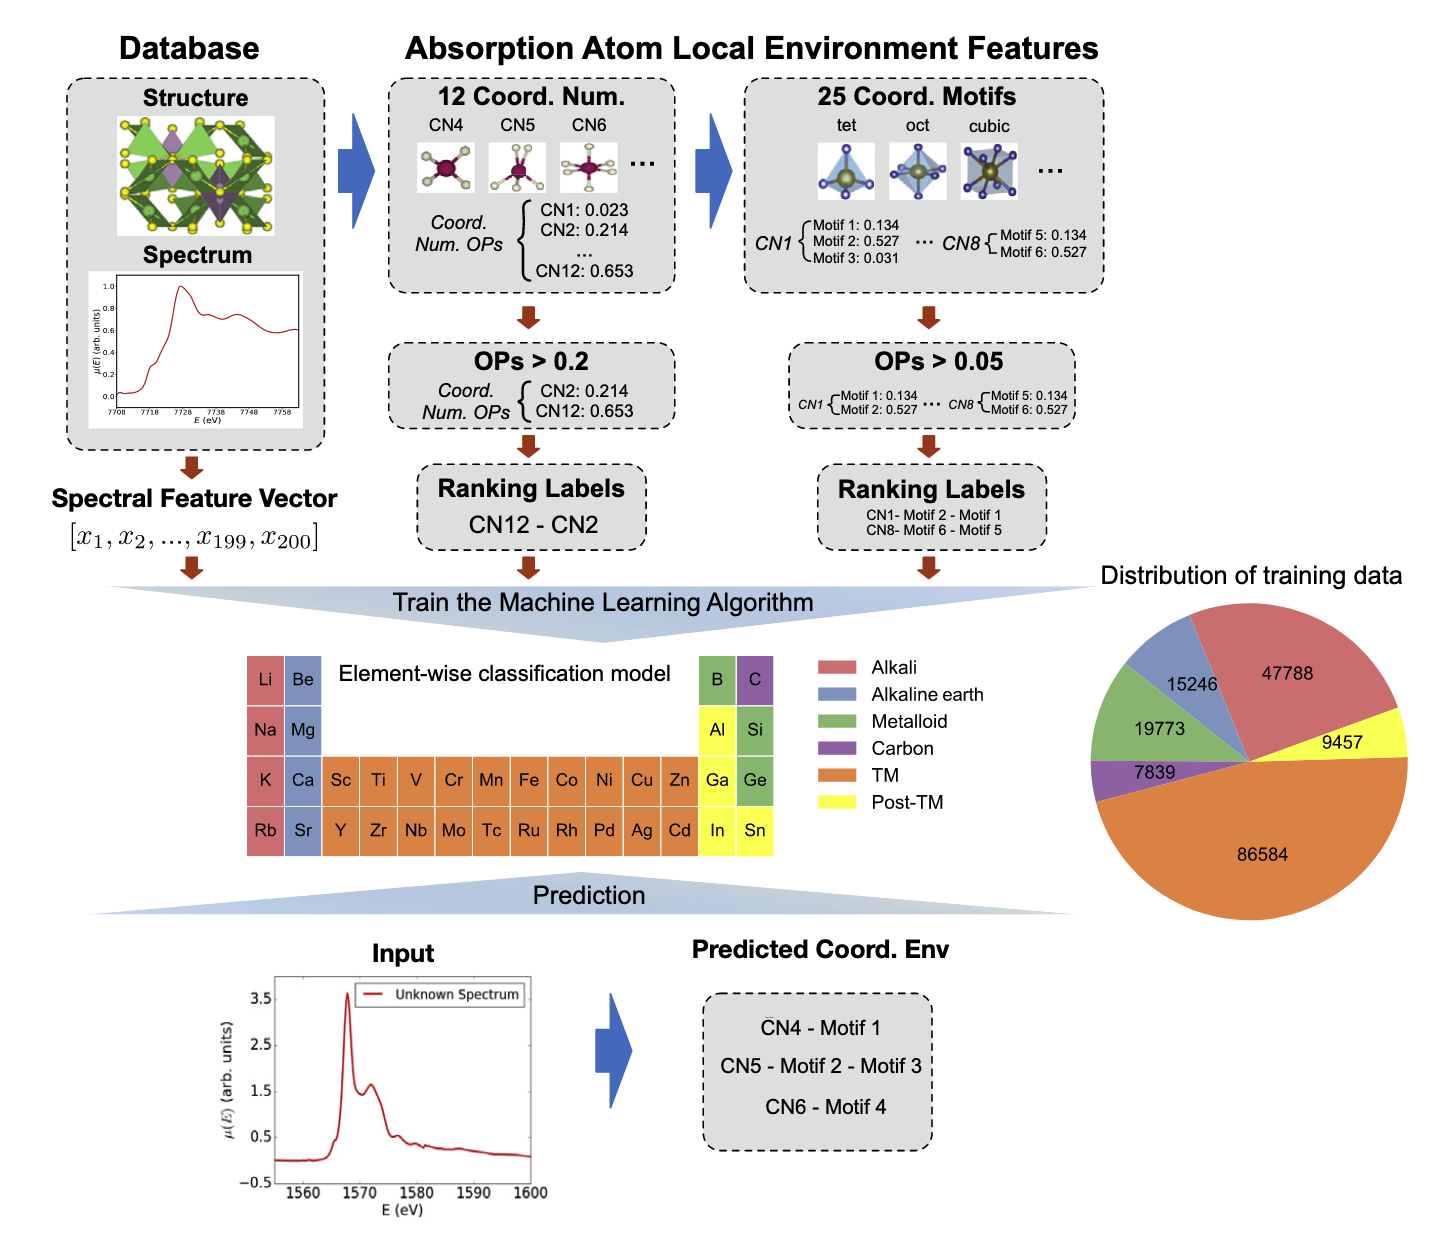
\includegraphics[width=0.45\textwidth]{figures/xasflowchart.png}
            \includegraphics[width=0.35\textwidth]{figures/xasaccuracy.png}
            \caption{Random Forest Coordination Environment Classification\cite{zhengRandomForestModels2020}}
        \end{figure}
    \end{frame}


    \begin{frame}{Other examples}
        \begin{figure}
            \centering
            \includegraphics[width=\textwidth]{figures/xrdclassification.png}
            \caption{X-ray diffraction data classification with CNNs\cite{oviedoFastInterpretableClassification2019}}
        \end{figure}
    \end{frame}

    \begin{frame}[allowframebreaks]{Bibliography}
        \bibliographystyle{unsrt}
        \bibliography{refs2022}
    \end{frame}


    \begin{frame}
        \Huge{\centerline{The End}}
    \end{frame}

\end{document}

